%%
% This is an Overleaf template for presentations
% using the TUM Corporate Desing https://www.tum.de/cd
%
% For further details on how to use the template, take a look at our
% GitLab repository and browse through our test documents
% https://gitlab.lrz.de/latex4ei/tum-templates.
%
% The tumbeamer class is based on the beamer class.
% If you need further customization please consult the beamer class guide
% https://ctan.org/pkg/beamer.
% Additional class options are passed down to the base class.
%
% If you encounter any bugs or undesired behaviour, please raise an issue
% in our GitLab repository
% https://gitlab.lrz.de/latex4ei/tum-templates/issues
% and provide a description and minimal working example of your problem.
%%

%\makeatletter
%\def\input@path{{../beamer/}}
%\makeatother

\documentclass[
  german,            % define the document language (english, german)
  aspectratio=169,    % define the aspect ratio (169, 43)
  % handout=2on1,       % create handout with multiple slides (2on1, 4on1)
  % partpage=false,     % insert page at beginning of parts (true, false)
  % sectionpage=true,   % insert page at beginning of sections (true, false)
]{tumbeamer}


% load additional packages
\usepackage{booktabs}
\usepackage{graphicx}
\usepackage{tikz}
\usepackage{url}
\usepackage{pgfplots}
\usepackage{hyperref}
\usepackage{pmboxdraw}
\usepackage{float}
\usepackage{listings}
\usepackage{circuitikz}
%\usepackage[european]{circuitikz}
\usepackage{babel}[ngerman]
\usepackage{csquotes}[autostyle]
\usepackage[useregional]{datetime2}

% image path
\graphicspath{ {./resources/} }

% presentation metadata
\title{Übung 09: Pipelining}
\subtitle{Einführung in die Rechnerarchitektur}
\author{Niklas Ladurner}

\institute{\theChairName\\\theDepartmentName\\\theUniversityName}
\date{\DTMdisplaydate{2023}{12}{15}{-1}}

\footline{\insertauthor~|~\insertshorttitle~|~\insertshortdate}


% macro to configure the style of the presentation
\TUMbeamersetup{
  title page = TUM tower,         % style of the title page
  part page = TUM toc,            % style of part pages
  section page = TUM toc,         % style of section pages
  content page = TUM more space,  % style of normal content pages
  tower scale = 1.0,              % scaling factor of TUM tower (if used)
  headline = TUM threeliner,      % which variation of headline to use
  footline = TUM default,         % which variation of footline to use
  % configure on which pages headlines and footlines should be printed
  headline on = {title page},
  footline on = {every page, title page=false},
}

% available frame styles for title page, part page, and section page:
% TUM default, TUM tower, TUM centered,
% TUM blue default, TUM blue tower, TUM blue centered,
% TUM shaded default, TUM shaded tower, TUM shaded centered,
% TUM flags
%
% additional frame styles for part page and section page:
% TUM toc
%
% available frame styles for content pages:
% TUM default, TUM more space
%
% available headline options:
% TUM empty, TUM oneliner, TUM twoliner, TUM threeliner, TUM logothreeliner
%
% available footline options:
% TUM empty, TUM default, TUM infoline


\begin{document}

\maketitle

\begin{frame}[c]{}{}
  \begin{center}
    \LARGE  Durchzählen!
  \end{center}
\end{frame}

\begin{frame}[c]{}{}
  \begin{center}
    \LARGE  Keine Garantie für die Richtigkeit der Tutorfolien: Bei Unklarheiten/Unstimmigkeiten
    haben VL/ZÜ-Folien Recht!
  \end{center}
\end{frame}

\begin{frame}[fragile, c]{Pipelining}{}
  \begin{itemize}
    \item Parallele Verarbeitung von mehreren Instruktionen
    \item Aufteilung der Instruktionsverarbeitung in 5 Teilschritte: Fetch, Decode, Execute, Memory, Writeback
    \item Daten- und Kontrollpfad des Prozessors wird in Stücke geteilt: Register zur Zwischenspeicherung dazwischen
    \item maximaler Speedup: Anzahl Pipelinestufen, Effekt bei großer Anzahl an Instruktionen erkennbar
  \end{itemize}

\end{frame}

\begin{frame}[fragile, c]{Pipelining}{}
  \begin{center}
    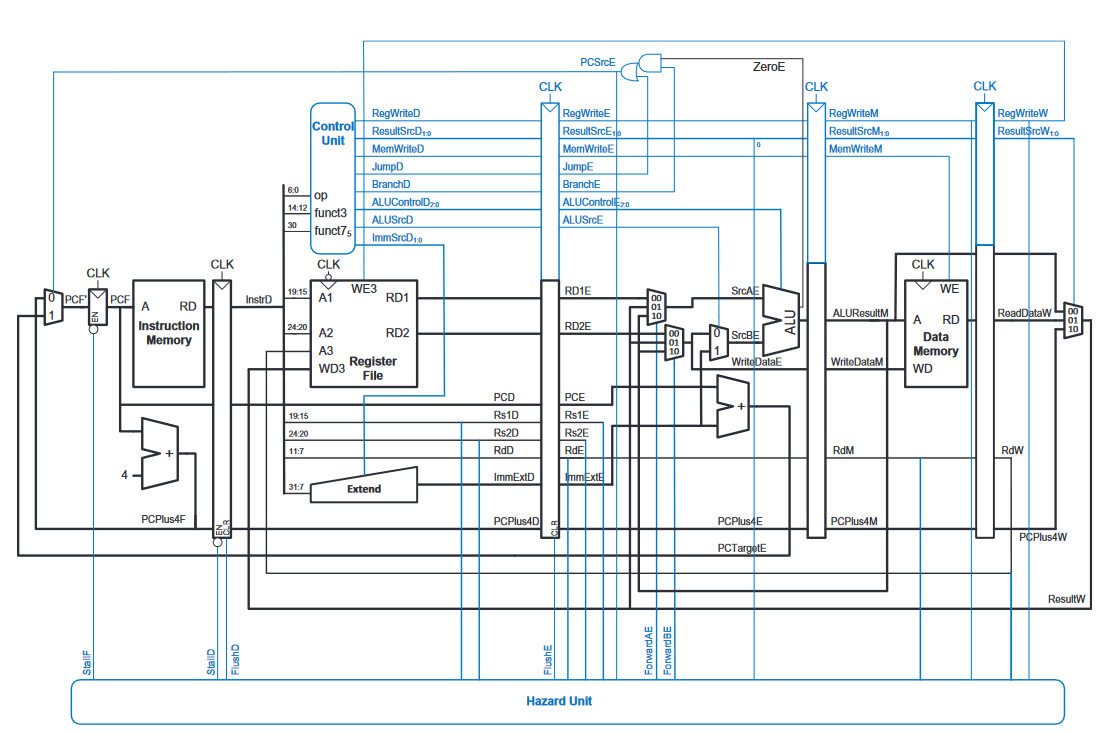
\includegraphics[width=0.7\textwidth]{w09_pipelined.png}
  \end{center}
\end{frame}


\begin{frame}[c, fragile]{Abhängigkeiten und Konflikte}{}
  \begin{itemize}
    \item Daten\textbf{abhängigkeiten}: RAW, WAR, WAW
    \item Pipelinekonflikte: Datenkonflikte (data hazards) und Steuerkonflikte (control hazards)
    \item Daten\textbf{konflikte} nur bei RAW möglich
    \item Steuerkonflikte bei Änderung der Kontrollflusses
  \end{itemize}
\end{frame}

\begin{frame}[c, fragile]{Lösung von Konflikten}
  Bei data hazards müssen mindestens \textbf{3 Befehle} zwischen zwei Instruktionen mit RAW-Abhängigkeit stehen:
  \begin{itemize}
    \item NOPs (Stalling)
    \item Befehlsumordnung (ohne Semantikänderung)
    \item Forwarding: noch nicht zurückgeschriebenes Ergebnis kann von der ALU direkt an den nächsten Befehl gegeben werden, falls dieser das Ergebnis benötigt
  \end{itemize}
  \vspace{0.5cm}
  Bei control hazards müssen mindestens \textbf{2 Befehle} zwischen der Sprungentscheidung und möglicherweise falsch geladenen Instruktion stehen.
  \begin{itemize}
    \item NOPs (Stalling)
    \item Branch Prediction (statisch/dynamisch): Falls Vorhersage falsch, müssen geladene Instruktionen entfernt werden
  \end{itemize}
  \vspace{0.5cm}
  weitere Konzepte: Out-of-Order-Execution, Register Renaming, \ldots
\end{frame}

\begin{frame}[c]{}{}
  \begin{center}
    \LARGE Fragen?
  \end{center}
\end{frame}

\begin{frame}[c, fragile]{Artemis-Hausaufgaben}{}
  \begin{itemize}
    \item H09 - Pipeline-Konflikte bis 07.01.2024 23:59 Uhr
    \item recht aufwendig, die Semantik des Programms darf nicht verändert werden!
    \item B01 - Concat bis 14.01.2024 23:59 Uhr
    \item Bonusaufgabe: 10 Punkte, ersetzt also eine ganze andere Aufgabe!
  \end{itemize}
\end{frame}

\begin{frame}[fragile, c]{Links}{}
  \begin{itemize}
    \item Zulip: \href{https://zulip.in.tum.de/#narrow/stream/1917-ERA-Tutorium---Mi-1600-MI4}{\enquote{ERA Tutorium - Mi-1600-MI4}}
    bzw. \href{https://zulip.in.tum.de/#narrow/stream/1940-ERA-Tutorium---Fr-1100-MW2}{\enquote{ERA Tutorium - Fr-1100-MW2}}
    \item \href{https://github.com/logisim-evolution/logisim-evolution/releases}{Logisim Evolution}
    \item \href{https://courses.edx.org/assets/courseware/v1/f06a2dc0c856f60ec0711e9f5e1c98cf/asset-v1:HarveyMuddX+ENGR85B+1T2023+type@asset+block/FinalReferences.pdf}{Referenztabellen (offizielle Tabellen sind auf den Übungblättern)}
  \end{itemize}
\end{frame}

\maketitle

\end{document}
